%%
%% This is file `example.tex',
%% generated with the docstrip utility.
%%
%% The original source files were:
%%
%% coppe.dtx  (with options: `example')
%% 
%% This is a sample monograph which illustrates the use of `coppe' document
%% class and `coppe-unsrt' BibTeX style.
%% 
%% \CheckSum{1417}
%% \CharacterTable
%%  {Upper-case    \A\B\C\D\E\F\G\H\I\J\K\L\M\N\O\P\Q\R\S\T\U\V\W\X\Y\Z
%%   Lower-case    \a\b\c\d\e\f\g\h\i\j\k\l\m\n\o\p\q\r\s\t\u\v\w\x\y\z
%%   Digits        \0\1\2\3\4\5\6\7\8\9
%%   Exclamation   \!     Double quote  \"     Hash (number) \#
%%   Dollar        \$     Percent       \%     Ampersand     \&
%%   Acute accent  \'     Left paren    \(     Right paren   \)
%%   Asterisk      \*     Plus          \+     Comma         \,
%%   Minus         \-     Point         \.     Solidus       \/
%%   Colon         \:     Semicolon     \;     Less than     \<
%%   Equals        \=     Greater than  \>     Question mark \?
%%   Commercial at \@     Left bracket  \[     Backslash     \\
%%   Right bracket \]     Circumflex    \^     Underscore    \_
%%   Grave accent  \`     Left brace    \{     Vertical bar  \|
%%   Right brace   \}     Tilde         \~}
%%
\documentclass[msc,numbers]{coppe}
\usepackage{amsmath,amssymb}
\usepackage[table]{xcolor}
\usepackage{hyperref}

\makelosymbols
\makeloabbreviations

\begin{document}
  \title{Estudo dos efeitos da corrente do brasil nas ondas da regi\~ao sul-sudeste}
  \foreigntitle{Study of brazil current effects on ocean waves within southeastern region}
  \author{Adriano}{Wiermann Barroso}
  \advisor{Prof.}{Nelson}{Violante Carvalho}{D.Sc.}
  \advisor{Ph.D.}{Pedro}{Veras Guimar\~aes}{Ph.D.}

  \examiner{Prof.}{Claudio Neves}{D.Sc.}

  \department{PENO}
  \date{03}{2019}

  \keyword{Primeira palavra-chave}
  \keyword{Segunda palavra-chave}
  \keyword{Terceira palavra-chave}

  \maketitle

  \dedication{A algu\'em cujo valor \'e digno desta dedicat\'oria.}

  \chapter*{Agradecimentos}

  Gostaria de agradecer a todos.

  \begin{abstract}
    
    Os efeitos de correntes superficiais em ondas s\~ao amplamente conhecidos, quando estas 
    est\~ao sujeitas a um campo de correntes existe uma troca de energia entre a onda
    e a corrente. Em casos de alto cizalhamento horizontal do campo de corrente \'e
    mais not\'avel estes efeitos. O presente trabalho tem como principal objetivo 
    analisar o efeito da Corrente do Brasil no campo de ondas na regi\~ao sul-sudeste
    do Brasil. Para isso foram escolhidos alguns eventos para estudo de caso em que 
    a Corrente do Brasil apresentava estruturas de mesoescala (meandros e v\'ortices).
    Estes eventos foram simulados atrav\'es de modelagem num\'erica com o modelo de ondas
    Wave Watch III com o campo de correntes provenientes do modelo Hycom. Foram empregadas
    simula{\c c}\~oes com e sem o campo de correntes afim de verificar os impactos.
    
  \end{abstract}

  \begin{foreignabstract}
		Abstract here...
  \end{foreignabstract}

  \tableofcontents
  \listoffigures
  \listoftables
  \printlosymbols
  \printloabbreviations

  \mainmatter
  \chapter{Introdu{\c c}\~ao}
  
  A an\'alise e modelagem num\'erica de correntes oce\^anicas e ondas foram historicamente desenvolvidas separadamente. No entanto, \'e bem conhecido os efeitos de correntes superficiais nas ondas, muitos trabalhos j\'a investigaram os efeitos que ocorrem nas ondas quando estas est\~ao sujeitas a um campo de correntes em larga escala. Trabalhos que fizeram essa an\'alise em sub e mesoescala s\~ao mais escassos, no entanto, regi\~oes como a corrente das Agulhas e corrente do Golfo j\'a foram estudados estes efeitos. Embora sejam os mesmos princ\'icios f\'isicos empregados, o impacto de correntes de menor escala ainda foi pouco explorado no oceano aberto \citet{Ardhuin2017}.
  
  Segundo conclus\~oes de \citet{Holthuijsen} em oceano aberto os efeitos locais das correntes podem ser consider\'aveis, por conta dos processos de gera{\c c}\~ao e dissipa{\c c}\~ao de onda serem mais afetados nessa regi\~ao.
	 
	A forma de intera{\c c}\~ao	de correntes com as ondas \'e atrav\'es da tens\~ao de radia{\c c}\~ao e em casos que o cisalhamento horizontal do campo de corrente \'e diferente de 0, ou seja n\~ao uniforme, ocorre maior troca de energia entre as ondas e a corrente atrav\'es dos termos de fluxo de momento \citet{Crapper1984}. Os principais locais em que este gradiente \'e diferente de zero s\~ao em correntes contorno oeste pois devido a sua maior intensidade, instabilidades da corrente como meandros e v\'ortices ocorrem com maior frequ\^encia.
	
	No Brasil a CB de contorno oeste se origina em latitudes pr\'oximas a 15$^o $S flui em dire{\c c}\~ao ao sul at\'e a regi\~ao da conflu\^encia brasil-malvinas pr\'oximo de 28$^o $S, ela se intensifica a medida que flui para baixas latitudes, com velocidades de corrente que alcan{\c c}am a ordem de 1 $m s^{-1}$ \citet{DaSilveira2008} e com intensa atividade de mesoescala bastante reportada na literatura.
	
	Apesar da exist\^encia de uma corrente de contorno oeste intensa e com atividade de mesoescala conhecida, ainda n\~ao h\'a na literatura estudos que investiguem a influ\^encia da CB no campo de ondas na regi\~ao sul-sudeste. O clima de ondas nesta regi\~ao \'e muito caracter\'istico com persist\^encia das vagas de nordeste geradas pelo AAS (Anticiclone do Atl\^antico Sul) e a chegada de algumas ondula{\c c}\~oes de sudoeste com longos per\'iodos oriundas de ciclones extratropicais, apresentando a bimodalidade do mar muito constante na regi\~ao \citet{Ricardo2009}.
  
  No estudo recente de \citet{Ardhuin2017} eles analisaram a influ\^encia da corrente do Golfo no campo de ondas. Pode-se verificar uma grande diferen{\c c}a no campo de ondas nas simula{\c c}\~oes com (\autoref{fig:fabrice}a) e sem corrente Golfo (\autoref{fig:fabrice}b).
  
	\begin{figure}[h]
		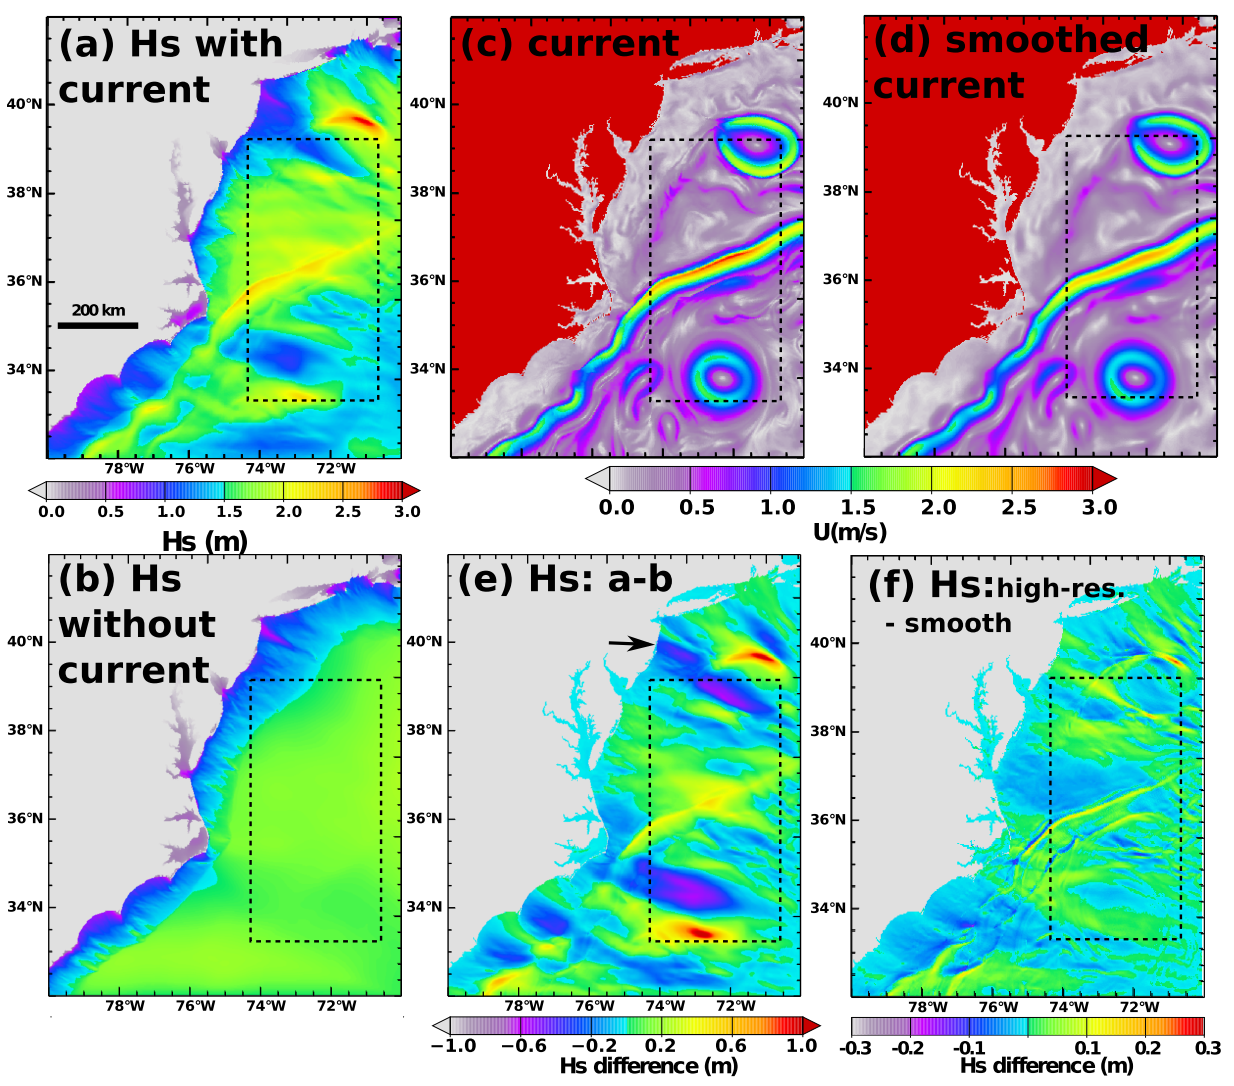
\includegraphics[height=14cm]{images/fabrice_hs.png}
		\caption{Imagem retirada do artigo citado. Impacto da corrente do Golfo nas ondas do tipo swell em 18 de Setembro de 2014, 6:00 UTC. Mapas de (a) altura de onda modelada com corrente, (b) altura de onda do modelo sem corrente, (c) corrente de alta resolu{\c c}\~ao do ROMS (d) mesma corrente filtrada. (e,f) diferen{\c c}a na altura de onda para (e) caso com corrente de alta resolu{\c c}\~ao menos caso sem corrente e (f) caso com corrente de alta resolu{\c c}\~ao menos caso com corrente filtrada. A \'area pontilhada refere-se a regi\~ao usada para an\'alise espectral.}
		\label{fig:fabrice}
		\centering
	\end{figure}
  
  Foram feitas simulac\~oes num\'ericas com o modelo de ondas Wave Watch III com dados de campo de corrente superficiais provenientes do modelo Hycom. Foram escolhidos eventos de alta instabilidade da CB para serem analisados.

  \chapter{Revis\~ao Bibliogr\'afica}

  Para ilustrar a completa ades\~ao ao estilo de cita{\c c}\~oes e listagem de
  refer\^encias bibliogr\'aficas, a Tabela~\ref{tab:citation} apresenta cita{\c
  c}\~oes de alguns dos trabalhos contidos na norma fornecida pela CPGP da
  COPPE, utilizando o estilo num\'erico.

  \begin{table}[h]
  \caption{Exemplos de cita{\c c}\~oes utilizando o comando padr\~ao
    \texttt{\textbackslash cite} do \LaTeX\ e
    o comando \texttt{\textbackslash citet},
    fornecido pelo pacote \texttt{natbib}.}
  \label{tab:citation}
  \centering
  {\footnotesize
  \begin{tabular}{|c|c|c|}
    \hline
    Tipo da Publica{\c c}\~ao & \verb|\cite| & \verb|\citet|\\
    \hline
    Livro & \cite{book-example} & \citet{book-example}\\
    Artigo & \cite{article-example} & \citet{article-example}\\
    Relat\'orio & \cite{techreport-example} & \citet{techreport-example}\\
    Relat\'orio & \cite{techreport-exampleIn} & \citet{techreport-exampleIn}\\
    Anais de Congresso & \cite{inproceedings-example} &
      \citet{inproceedings-example}\\
    S\'eries & \cite{incollection-example} & \citet{incollection-example}\\
    Em Livro & \cite{inbook-example} & \citet{inbook-example}\\
    Disserta{\c c}\~ao de mestrado & \cite{mastersthesis-example} &
      \citet{mastersthesis-example}\\
    Tese de doutorado & \cite{phdthesis-example} & \citet{phdthesis-example}\\
    \hline
  \end{tabular}}
  \end{table}

  \chapter{M\'etodo Proposto}
  \chapter{Resultados e Discuss\~oes}
  \chapter{Conclus\~oes}

  \backmatter
  \bibliographystyle{coppe-unsrt}
  %\bibliographystyle{apa}
  \bibliography{mestrado}

  \appendix
  \chapter{Algumas Demonstra{\c c}\~oes}
\end{document}
%% 
%%
%% End of file `example.tex'.
